
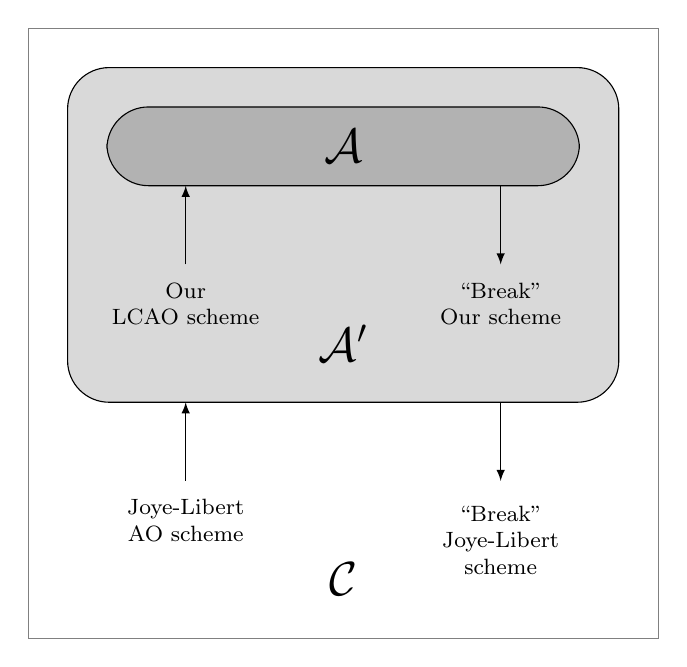
\begin{tikzpicture}[font=\footnotesize]
% Bounding box
\draw [gray] (0,-0.25) rectangle (8,7.5);

% Outer adversary rectangle
\draw[rounded corners=15pt, fill=gray!30] (0.5,7) rectangle (7.5,2.75);
% Inner adversary rectangle
\draw[rounded corners=15pt, fill=gray!60] (1,6.5) rectangle (7,5.5);

% Adversaries and challenger
\node at (4,3.5) {\LARGE$\mathcal{A}'$};
\node at (4,6) {\LARGE$\mathcal{A}$};
\node at (4,0.5) {\LARGE$\mathcal{C}$};

% Arrows
\node[text width=3cm, align=center] at (2,1.25) {Joye-Libert\\AO scheme};
\draw [-latex] (2,1.75) -- (2,2.75);

\node[text width=3cm, align=center] at (2,4) {Our\\LCAO scheme};
\draw [-latex] (2,4.5) --(2,5.5);

\node[text width=3cm, align=center] at (6,4) {``Break''\\Our scheme};
\draw [-latex] (6,5.5) -- (6,4.5);

\node[text width=3cm, align=center] at (6,1) {``Break''\\Joye-Libert\\scheme};
\draw [-latex] (6,2.75) -- (6,1.75);

\end{tikzpicture}